

% Definitionen



%%%%%%%%%% Kopfbereich %%%%%%%%%%%%%
%\documentclass[a4paper,titlepage,oneside,fontsize=2pt]{scrbook} % Dokumentklasse
\documentclass[11pt,a4paper,titlepage,oneside]{report} % Dokumentklasse
\pdfminorversion=7  %akzeptiert pdf in version 1.7
%\RequirePackage{pdf14}
\usepackage{etex}

\usepackage{nomencl,longtable,ifthen} % Symbolverzeichnis
%\usepackage{ngerman} % Deutsch, neue Rechtschreibung
%\usepackage[latin1]{inputenc} % Sonderzeichen ��� etc.
\usepackage[T1]{fontenc} % T1 Format
\usepackage{geometry} % Seitenr�nder
\usepackage[printonlyused]{acronym} % Abk�rzungsverzeichnis
\usepackage{graphicx} % Einbinden von Grafiken
\usepackage{fancyhdr} % Gestaltung von Kopf- und Fu�zeile
%\usepackage{bibgerm} % Literaturverzeichnis
%\usepackage[squaren]{SIunits} % SI Einheiten
\usepackage{amsmath, amsthm, amssymb}
\usepackage{mathtools}
\usepackage{floatflt}
\usepackage{float}
\usepackage{graphics}
\usepackage{picins}
\usepackage{wrapfig}
\usepackage{threeparttable}
\usepackage{textcomp}
\usepackage{tabularx}
\usepackage{hhline}
\usepackage{siunitx}
\usepackage{framed, color}

\usepackage{courier}
\usepackage{listings}
\usepackage{color}
\usepackage{multicol}
\usepackage{multirow}
\usepackage[hyphens]{url}
\usepackage{xcolor}
\usepackage[right]{eurosym}
\usepackage{colortbl}
\usepackage{subfigure}
\usepackage{setspace}
\usepackage{footnote}
\usepackage{wasysym}
% Seitenstil definieren
\pagestyle{fancy}
\fancyhead{}
\fancyfoot{}
\rhead{\leftmark}
\cfoot{\thepage}
\renewcommand{\headrulewidth}{0pt}
\renewcommand{\footrulewidth}{0.4pt}

\usepackage[bottom]{footmisc}
%\usepackage{footmisc}
\setlength{\footnotemargin}{2mm} % Einr�cken der Fu�note
\setlength{\footnotesep}{12pt}% Abstand zwischen den Fu�noten 
\setlength{\skip\footins}{22pt}% Abstand Zwischen Haupttext und Fu�noten

%-------------------------------
\usepackage{calc}

% Paket f�r Zeichnungen
\usepackage{tikz}
\usepackage{tikz-timing}
\usepackage{vhistory}
%

\usetikztiminglibrary[new={char=Q,reset char=R}]{counters}
\usetikztiminglibrary{arrows}
\usetikzlibrary{shapes,
								arrows,
								calc,
								automata,
								positioning,
								mindmap,
								fit,
								trees,
								shadows,
								decorations,
								scopes,
								matrix,
								chains,
								shapes.misc,% wg. rounded rectangle
  							shapes.arrows,%
  							decorations.pathmorphing}



%-------------------------------
\usepackage[plainpages=false]{hyperref}
\hypersetup{colorlinks%Rot im inhaltsverzeichniss entfernt"'
,linkcolor=black
,filecolor=blue
,urlcolor=blue
,citecolor=blue}

%\pdfoptionpdfminorversion=6
%\pdfminorversion=7  %akzeptiert pdf in version 1.7
\setcounter{tocdepth}{3} %%f�r subsubsection!!!
\setcounter{secnumdepth}{3} 
%\usepackage{watermark}
\definecolor{light}{gray}{.50}



%%%%%%%%% Neue Kommandos %%%%%%%%%%%%%
\let\abk\nomenclature % Abk�rzung shortcut
\newcommand{
\changefont}[3]{\fontfamily{#1} \fontseries{#2} \fontshape{#3} \selectfont} % Setzen der Schriftart



%%%%%%%%%%%%%% zus�tzliche unit-Spalte %%%%%%%%%%%%%%%%
\newcommand{\nomunit}[1]{%
\renewcommand{\nomentryend}{\hspace{2em}\hspace*{\fill}#1}}


%%%%%%%%%%%%%% longtable an Stelle der Liste %%%%%%%%%%
\makeatletter
\def\@@@nomenclature[#1]#2#3{%
   \def\@tempa{#2}\def\@tempb{#3}%
   \protected@write\@nomenclaturefile{}%
      {\string\nomenclatureentry{#1\nom@verb\@tempa @{\nom@verb\@tempa}&%
         \begingroup\nom@verb\@tempb\protect\nomeqref{\theequation}%
            |nompageref}{\thepage}}%
   \endgroup
   \@esphack}
\def\thenomenclature{%
   \@ifundefined{chapter}{\section*}{\chapter*}{\nomname}%
   \nompreamble
   \begin{longtable}[l]{@{}ll@{}}}
\def\endthenomenclature{%
\end{longtable}
\nompostamble}
\makeatother


%%% Listings
\definecolor{LinkColor}{rgb}{0,0,0.5}
\definecolor{ListingBackground}{rgb}{0.9,0.9,0.9}
\definecolor{dunkelgrau}{rgb}{0.8,0.8,0.8}
\definecolor{lightblue}{rgb}{0.6132,0.7382,0.8554}
\definecolor{lightwhite}{rgb}{1,1,1}
\definecolor{schwarz}{rgb}{0,0,0}
\definecolor{weiss}{rgb}{1,1,1}
\definecolor{codegreen}{rgb}{0,0.5,0}
\definecolor{codegray}{rgb}{0.0,0.5,0.5}
\definecolor{codepurple}{rgb}{0.5,0,0.5}
\definecolor{backcolour}{rgb}{0.95,0.95,0.92}


\lstloadlanguages{C} % TeX sprache laden, notwendig wegen option 'savemem'
\lstset{%
	language=C,     				% Sprache des Quellcodes ist TeX
commentstyle=\color{codegreen},
    keywordstyle=\color{blue}\bfseries,
    numberstyle=\tiny\color{codegray},
    stringstyle=\color{codepurple},
	numbers=left,            % Zelennummern links
	stepnumber=1,            % Jede Zeile nummerieren.
	numbersep=5pt,           % 5pt Abstand zum Quellcode
	numberstyle=\tiny,       % Zeichengr�sse 'tiny' f�r die Nummern.
	breaklines=true,         % Zeilen umbrechen wenn notwendig.
	breakautoindent=true,    % Nach dem Zeilenumbruch Zeile einr�cken.
	postbreak=\space,        % Bei Leerzeichen umbrechen.
	tabsize=2,               % Tabulatorgr�sse 2
	basicstyle=\ttfamily\footnotesize, % Nichtproportionale Schrift, klein f�r den Quellcode
	showspaces=false,        % Leerzeichen nicht anzeigen.
	showstringspaces=false,  % Leerzeichen auch in Strings ('') nicht anzeigen.
	extendedchars=true,      % Alle Zeichen vom Latin1 Zeichensatz anzeigen.
	captionpos=b, %Caption unten
	backgroundcolor=\color{weiss}} % Hintergrundfarbe des Quellcodes setzen.


%%%%%%%%%%%%%%%%%%%%%%%%%%%%%%%%%%%%%%%%%%

\lstdefinelanguage{Assembler}%
   {morekeywords={BL,LDR,MOV,bx,sub,stmfd,ldr,str,mrs,msr,ldmia},%
    morekeywords=[2]{.global,.extern,.macro,.endm},%
    alsoletter={.,0,1,2,3,4,5,6,7,8,9},%
    alsodigit={?},%
    sensitive=false,%
    morestring=[b]",%
    morecomment=[s]{/*}{*/},%
    morecomment=[l]@,%
    morecomment=[l]//,%
   }[keywords,comments,strings]

%%%%%%%%% Erstellung der Verzeichnisse %%%%%%%%%%%%%
\makenomenclature
%\makeglossaries
%\makeindex

%%%%%%%%% Seitenlayout %%%%%%%%%%%%%
\setlength{\parindent}{0pt} % Zeileneinzug bei Absatz
\linespread{1.3} % hor. Zeilenabstand
%\geometry{a4paper, top=40mm, left=35mm, right=25mm, bottom=40mm, headsep=10mm, footskip=10mm} % Randabst�nde kl�ren

\geometry{a4paper, top=40mm, left=30mm, right=30mm, bottom=40mm, headsep=10mm, footskip=10mm} % Randabst�nde kl�ren
\setlength{\headheight}{15pt}

 % Include Packages

% to fix grouping in the list of .......
\let\Chapter\chapter
\def\chapter{\addtocontents{lol}{\protect\addvspace{10pt}}\Chapter}

%%%%%%%%% Dokumentenbeginn %%%%%%%%%%%%%%%
\begin{document}


\title{TITLE}
\author{NAME}

%\nomenclature[gz]{}{\nomunit{}}
%\changefont{cmr}{m}{n},
%\fontsize{12}{15}
%\selectfont


%Titelseite
\pagenumbering{Alph}

%%%%%%%% Titelseite %%%%%%%%%%%%%
\begin{titlepage}
\newgeometry{top=40mm, left=33mm, right=23mm, bottom=40mm}
\begin{center}

\begin{table}              
\begin{tabular}{ll}

\includegraphics[width=6cm]{images/logo_hse.jpg} %& \includegraphics[height=1cm]{images/weiss.pdf}\\�
%%& \includegraphics[width=5cm]{images/weiss.pdf}\\ \\ \\
\end{tabular}
\end{table}

\vspace*{2mm}
\begin{huge}
Project Work\\
\end{huge}

\vspace{17mm}

\begin{Huge}
{\sf \textsc{Oscilloscope to display values sent via UDP} }\\
\end{Huge}

\vspace{37mm}

\onehalfspacing
\large{Vikas Agrawal}\\
%\large{geboren am 02.03.1990}\\
%\large{Poststra�e 8}\\
%\large{72587 R�merstein}\\
\end{center}
\onehalfspacing
\vspace{5mm}

\begin{center}
\doublespacing
%\begin{tabbing}
%\large{Durchgef�hrt bei:} \= \large{\textsc{Robert Bosch GmbH}, Abteilung GS/ESC3}\\
%\>\large{Robert-Bosch-Str. 2, 71701 Schwieberdingen}\\
%\end{tabbing}

\singlespacing
\large{\textsc{Hochschule Esslingen}}\\
\large{{Faculty: Computer Science}}\\

\onehalfspacing
\vspace{15mm}
%\begin{tabbing}
%%\doublespacing
\large{Supervisor:  Prof. Friedrich}\\

\onehalfspacing
%\end{tabbing}

\vspace{10mm}
\large{Processing time: 01.08.2015 -  }\\
%\large{Fachhochschule Esslingen}\\
%\large{Semester: IT5B}\\
%\large{Fakult�t: Informationstechnik}\\
%\large{Schwerpunkt: Technische Informatik}\\
%\large{Matrikelnummer: 737788}\\
%\vspace{5mm}
%\large{Sperrvermerk: Firmenvertraulich}



\end{center}
\end{titlepage}
 % Erkl�rung
\restoregeometry % Manipulierte Seitenr�nder wiederherstellen.
\setcounter{page}{2}
\chapter*{}
\thispagestyle{empty}  % Leerseite mit Alpha Buchstaben


%%%%%%%%%% Externe Seiten %%%%%%%%%%%%%
%
%%%%%%%%%% Verzeichnisse, Erkl�rungen etc. %%%%%%%%%%%%%
%{
\pagestyle{plain} % Leere Seiten
%\include{parts/blankpage} % Leerseite
\pagenumbering{Roman} % R�mische Seitennummerierung f�r die ersten Seiten


%\include{parts/Sperrvermerk} % Sperrvermerk
%\include{parts/Erklaerung} % Erkl�rung
%\include{parts/Abstract} % Kurzfassung

%------------------
%Versioning page
%\begin{document}
% Start of the revision history table
\begin{versionhistory}
  \vhEntry{1.0}{01.08.15}{Vikas Agrawal}{created}
\end{versionhistory}
\pagebreak
%------------------

\pdfbookmark[1]{Table of contents}{toc} % PDF-Bookmark f�r Inhaltsverzeichnis setzen
\tableofcontents % Inhaltsverzeichnis
\clearpage


\chapter*{List of Abbreviations}											% Kapitel Abk�rzungsverzeichnis (ohne Nummerierung)
\markboth{List of Abbreviations}{List of Abbreviations}

\begin{acronym}[XXXXXXXXX]
%\renewcommand{\bflabel}[1]{\normalfont{\normalsize{#1}}\hfill}  %Serivenschrift
\setlength{\itemsep}{-\parsep}
	
%\singlespacing
  \acro{Abbreviation}{Description}
  \vspace{6mm}%\acro{}{}
	\acro{RTC}{Real Time Clock}

	%-----------------
	
\onehalfspacing
\end{acronym}
\addcontentsline{toc}{section}{List of Abbreviations}	% in Inhaltsverzeichnis aufnehmen



%\clearpage

%\include{parts/Symbolverzeichniss}
%\clearpage
%------------------------
%------------------------

\pagenumbering{arabic} % Arabische Seitennummerierung f�r den Hauptteil
\onehalfspacing

% Kapitelanfangsseiten umgestalten
\fancypagestyle{plain}{
\fancyhf{}
\cfoot{\thepage}\renewcommand{\headrulewidth}{0pt}} 


%%%%%%%%% Hauptteil %%%%%%%%%%%%%
\pagestyle{fancy}
%\include{parts/Einleitung}
\chapter{Task description}The task is to make a graphical user interface to display the values of the sensor that are received by the oscilloscope via the UDP protocol.


\chapter{Development Environment} 
\textbf{Coding Language}: The project is developed on Java Version 7. To download the version 7, simply do yum install java-1.7.0-openjdk. For the sake of simplicity, the Java Version 7 should also be available on Windows as well.\\\\
\textbf{Versioning}: The software is versioned via GIT and is secured on the remote server. The sensor oscilloscope can be cloned via git@atreus.informatik.uni-tuebingen.de:agrawal/sensoroscilloscope.git. To test the udp connection, a set of python scripts has been written and they should be also cloned by running the command git clone git@atreus.informatik.uni-tuebingen.de:agrawal/python\_scripts.git\\

\chapter{Executing the Software}
When the software is executed, the user needs to select the radio button UDP and press the start button. As soon as the button is pressed, a server is started and starts listening at the port number \textbf{9876} on the local host.\\
To test if the server was successfully started, run the command nmap localhost -p 0-10000. This will list all the open ports.\\
It is required to add the panels in the oscilloscope before sending test udpdata to the oscilloscope. If the entry of the port at 9876 is available, then run the python script udpsend.py. 




%\subsection{State space}\label{chapter_StateSpace}

In this section, the basic knowledge for understanding the so-called state space representation, is described. The state space representation is a mathematical system of a physical model. It consists of inputs and outputs and the state variables that are related to the differential equations of that model. One huge advantage of this idea is, that the Laplace transformation is not needed. Therefore the state space representation is also called 'time-domain approach'. Another opportunity is the usage of initial conditions and that a system can have nonlinear constraints. 

So the next step is to understand the state variables. As already mentioned, every state space system consists of inputs, outputs and state variables. These state variables describe the entire state of the system at any time. The simplest way to decide where to set the state variables, is to put them behind every single integrator block. So the state variable itself is behind this block and the corresponding derivative in front. \myfigref{fig:simpleProcess} shows a simple example for a third order system. This system is called a SISO system, that means 'Single Input Single Output'. In this case \textit{u} is the single input and \textit{y} the single output of the system. Besides, there are MIMO systems having 'Multiple Input Multiple Output'. Chapter \ref{chapter_MIMO} handles them.

\begin{figure}
	\centering
		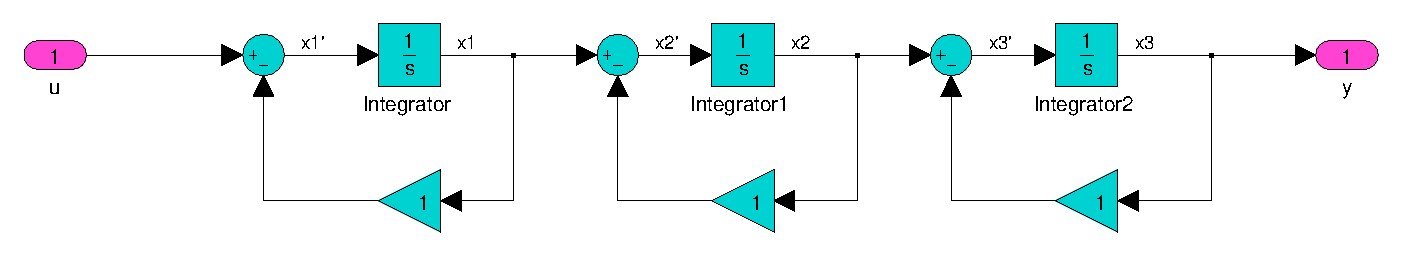
\includegraphics[width=1.00\textwidth]{03_Grafiken/simpleProcess.pdf}
	\caption{Simple example of a SISO process}
	\label{fig:simpleProcess}
\end{figure}

The differential equations for this system look like that:
\begin{align*}
	x1' & = -x1 + u\\ 
	x2' & = x1 - x2\\
	x3' & = x2 - x3\\
	y   & = x3
\end{align*}

These differential equations can be transformed into four matrices:
\begin{align}
\bordermatrix[{[]}]{
    & x1 & x2 & x3 & u \cr
x1' & \colorbox{yellow}{-1} & \colorbox{yellow}{0}  & \colorbox{yellow}{0}  & \colorbox{red}{1} \cr
x2' & \colorbox{yellow}{1}  & \colorbox{yellow}{-1} & \colorbox{yellow}{0}  & \colorbox{red}{0} \cr
x3' & \colorbox{yellow}{0}  & \colorbox{yellow}{1}  & \colorbox{yellow}{-1} & \colorbox{red}{0} \cr
y   & \colorbox{green}{0}   & \colorbox{green}{0}   & \colorbox{green}{1}   & \colorbox{cyan}{0}
}
\end{align}

The most important is the \colorbox{yellow}{A matrix}, called the 'state matrix'. This matrix declares the dependency between all state variables in the whole system. With this matrix it is possible to get information about the response characteristics and the stability of the system. The \colorbox{red}{B matrix} is called the 'input matrix', the \colorbox{green}{C matrix} is called the 'output matrix' and at least the \colorbox{cyan}{D matrix} is called the 'feedforward matrix'. 

In most cases - as well as in this project - there is no direct connection between an input and an output. Therefore the 'D matrix' is a zero matrix. The input matrix B describes the dependency of the state variables to the input vectors. This fact is needed later on, to decide whether the system is controllable or not. The output matrix C describes the same as the input matrix, but for the outputs. The C matrix is used to declare which states are observable.

Now two more terms are mentioned - controllability and observability. 

The controllability first. To achieve a required dynamic behavior of the process, it is necessary, that all of its state variables can be moved by the input independently from each other. 

\begin{align}\label{Q_s}
	Q_s = \left[b\ \  A*b\ \ A^2*b\ \ \cdots\ \ A^{n-1}*b\right]
\end{align}

According to Kalman, the controllability matrix $Q_s$ \myeqref{Q_s} has to be full rank of the whole system. This is the most important check in the beginning of any project about state space controlling. For the simple example process the controllability is given, because the rank of the $Q_s$ matrix is three and that system is third order. Figure \ref{fig:Steuerbarkeit} shows the controllability graphical.

\begin{figure}
	\centering
		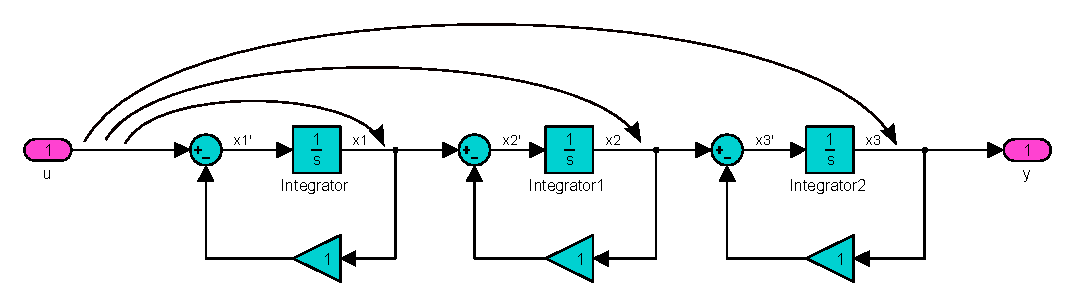
\includegraphics[width=1.00\textwidth]{03_Grafiken/Steuerbarkeit.pdf}
	\caption{Principle of controllability}
	\label{fig:Steuerbarkeit}
\end{figure}

The second term mentioned, is observability. It is very similar to the controllability, but it declares whether each state variable has influence on the output of the system.

\begin{align}\label{Q_b}
	Q_b = \left[c^T\ \  c^T*A\ \ c^T*A^2\ \ \cdots\ \ c^T*A^{n-1}\right]^T
\end{align}

The condition according to Kalman is very akin to the condition for controllability - the observability matrix $Q_b$ \myeqref{Q_b} must be full rank of the system. The rank of the $Q_b$ matrix in this example is three - so each state is observable. Figure \ref{fig:Beobachtbarkeit} shows the observability graphical.

\begin{figure}
	\centering
		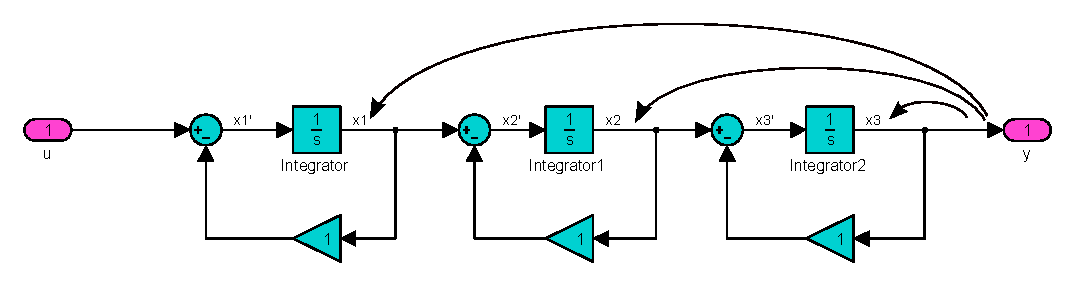
\includegraphics[width=1.00\textwidth]{03_Grafiken/Beobachtbarkeit.pdf}
	\caption{Principle of observability}
	\label{fig:Beobachtbarkeit}
\end{figure}




%\include{parts/Ausblick}



%\include{parts/Danksagung} % Danksagung



%%%%%%%%% Anhang, Literaturverzeichnis %%%%%%%%%%%%%
%\include{parts/anhang} % Anhang
%\include{parts/Software} % Software

%------------- Altes Abb. Verzeichnis in Gruppen
\phantomsection
\addcontentsline{toc}{chapter}{List of Figures}
\listoffigures % Bilderverzeichnis

\clearpage
\phantomsection
\addcontentsline{toc}{chapter}{List of Tables}
\listoftables % Tabellenverzeichnis}
\clearpage


\phantomsection
\addcontentsline{toc}{chapter}{List of Listings}
\renewcommand{\lstlistlistingname}{List of Listings}
%\renewcommand{\lstlistingname}{List of Listings}
\lstlistoflistings
\clearpage

%%\begingroup
%%\phantomsection
%%\addcontentsline{toc}{chapter}{\listfigurename}
%%\renewcommand*{\addvspace}[1]{}
%%\listoffigures
%%\cleardoublepage
%%\phantomsection
%%\addcontentsline{toc}{chapter}{\listtablename}
%%\listoftables
%%\endgroup

%------------- Altes Abb. Verzeichnis ohne Gruppen
%%\begingroup
%%\phantomsection
%%\addcontentsline{toc}{chapter}{\listfigurename}
%%\renewcommand*{\addvspace}[1]{}
%%\listoffigures
%%\cleardoublepage
%%\phantomsection
%%\addcontentsline{toc}{chapter}{\listtablename}
%%\listoftables
%%\endgroup

\phantomsection
\addcontentsline{toc}{chapter}{Bibliography}
\bibliography{Quellen}
\bibliographystyle{alpha}


\end{document}
% ENDE
